% 论文本体；保留原冻结预测、拟合、统计规则和不利结果。
\documentclass[UTF8,11pt]{ctexart}
\usepackage[margin=1in]{geometry}
\usepackage{amsmath,amssymb,booktabs,array,longtable,graphicx,xurl}
\usepackage[hidelinks]{hyperref}
\usepackage{tikz,placeins,needspace}
\usetikzlibrary{arrows.meta}
\setlength{\emergencystretch}{3em}
\newcommand{\R}{\mathbb{R}}
\newcommand{\ES}{\operatorname{ES}}
\newcommand{\supp}[1]{\href{supplement.pdf\##1}{科学补充材料}}
\newcommand{\audit}[1]{\href{audit-notes.pdf\##1}{审查记录}}
% Generated from original public aggregate values; no inference.
\newcommand{\FullES}{477.85}
\newcommand{\InertialES}{824.73}
\newcommand{\FullFDE}{1326.09}
\newcommand{\FullADE}{636.11}
\newcommand{\InertialDelta}{-346.87}
\newcommand{\PointRowFull}{Full & 73.77 & 332.31 & 812.26 & 1326.09\\}
\newcommand{\PointRowGMM}{GMM & 71.92 & 323.79 & 792.99 & 1299.11\\}
\newcommand{\PointRowdtThreeHundred}{dt300 & 75.88 & 340.10 & 825.76 & 1335.73\\}
\newcommand{\PointRowInertial}{Inertial & 31.17 & 237.93 & 934.03 & 2095.78\\}

\author{}
\date{公开审阅修订稿，2026年10月9日；署名待确认}

\title{概率运动预测的分时域表现与经验欠覆盖}
\begin{document}
\maketitle
\begin{abstract}
本文研究已拟合随机运动预测器的分布评分、位置准确性与不确定性覆盖之间的关系。
评估使用按时间与未来真实路线地图支持事后筛选的46个独特记录哈希块、
五个固定模拟种子与512个粒子。预测时域为保存时钟下名义1、5、15和30分钟；
物理时钟来源与参与者独立性尚未确立，评估队列也不是此前未接触的留出集。
Full的四目标等权能量评分（ES）为\FullES\ 米，确定性恒速惯性参考为
\InertialES\ 米。1和5分钟惯性更好，15和30分钟Full更好。
Full的30分钟名义90\%边际预测圆实际仅覆盖46.52\%的目标。
原21项主方法比较得到14项有限算法实际等价与七项证据不足状态；
没有区间整体越过登记实际意义界的效果，全部分辨率不变判断仍为证据不足。
必需预测失败使地形家族推断不可用，这不等于地形无效。
这些条件性发现支持同时报告评分、均值位置误差、覆盖和证据可用性，
而不是部署可靠性承诺或算法的普遍排名。
\end{abstract}

\noindent\textit{证据版本。}原一次保存输出审计与固定预算公开汇总复算已完成。
本次重组不改变预测、拟合或统计规则。完整科学规格和全量表见
\supp{sec:models}，版本、执行及回应历史见\audit{sec:audited-review-update}。
署名、路线公开许可与人类验收是另外的决定。

\section{引言与研究范围}\label{sec:introduction}\hypertarget{sec:introduction}{}
运动预测需要给出合理的未来位置，同时使不确定性可见。较低分布评分、较小位置误差
与达到标称覆盖的区域回答不同问题，不一定共同改善。本文以有限的可解释拟合随机
预测器检查这种区别，而不是提出新的通用随机微分方程（SDE）理论。

连续时间相关随机游走处理不规则观测与运动持续性\cite{johnson2008}。
切换状态空间模型描述潜在模式\cite{ghahramani2000}，但跨批次迁移参数时必须
审视模式身份。整合步长选择联系运动与环境选择\cite{avgar2016,avgar2017correction}，
这类关系不能由任意且不平衡的特征消融自动识别。
学习式轨迹模型\cite{gupta2018,salzmann2020}与神经SDE路径生成器\cite{kidger2021}
提供研究背景，不是本实验已执行的性能基线。
可解释随机系统辨识\cite{gao2024}支持显式列出漂移与噪声规格。
本文的贡献是对实际评估预测器的分时域取舍与欠覆盖作有边界的经验检查。

恰当评分规则\cite{gneiting2007,gneiting2008}评价预测分布与实现目标，
却不能认证某个边际区域达到名义覆盖。因此ES、粒子均值误差、预测圆覆盖与面积
分别报告。惯性参考先建立短长时域反转，内部比较再解释哪些实施程序改变这些诊断。
它们不能证明复杂随机模型相对于简单概率运动基线是必要的。

原登记问题保持可追溯：RQ1考察方法组件比较，RQ2考察历史基线之上的地形配置增量。
RQ1现在给出条件性固定算法结果，但部分比较同时改变多个因素或共享参数。
RQ2保留设计和明确的不可用结果，而不是地形正效应或零效应答案。
本文以证据实际能够支持的发现组织论证。

\section{预测器与比较实际改变的内容}\label{sec:models}\hypertarget{sec:models}{}
\subsection{普通Full与实际输入}
令$X=(X_e,X_n)^\top$为保存局部坐标框架中的位置（米），$t$为保存时间坐标（秒）。
起点为最后一个允许的前缀位置，首个可见位置锚定坐标框架。
普通Full有三个拟合模式，位置动力学为
\begin{equation}\label{eq:ordinary-full}
 dX_t=\Theta_{m_t}^{\top}\psi(X_t,t)\,dt+L_{m_t}\,dW_t,
 \quad\psi=(1,X_e,X_n,S)^\top,\quad L_mL_m^\top=Q_m=\tau R_m.
\end{equation}
$\Theta_m$给出米/秒漂移，$S$为由保留绝对tick计算的太阳／日历输入\cite{noaa}，
$R_m$为位移率残差协方差（米$^2$/秒$^2$）。转换为$Q_m$使用模型观测间隔
$\tau$，不是积分步长$h$。秒与日光的物理解释仍取决于时钟来源（第\ref{sec:data}节）。
保存混合概率$\pi_m$来自拟合与适应混合，不是新前缀下更新的模式后验。
各粒子在起点按保存$\pi$初抽模式。段固定Full保持该初抽；只有切换路线在各自$\tau$
事件重抽，不在每个积分子步或评分输出重抽。

\begin{table}[htbp]\centering
\caption{预测器真正使用的前缀信息。更新了缓冲区不等于漂移读取该信息；三条路线不能互换。}
\label{tab:inputs}
\begin{tabular}{p{.20\linewidth}p{.72\linewidth}}\toprule
路线 & 漂移输入与解释\\\midrule
普通Full & 位置、日历代理与保存$\pi$；固定坐标框架、位置、时钟及随机流后，不读初速度或近期带符号方向。\\
显式特征 & 速率范数与位置径向方向；同时由三模式变单模式。径向方向不是速度方向。\\
地形base/full & 割线速度与三位置带符号历史；all-terrain再加入保留地图特征。\\\bottomrule
\end{tabular}\end{table}
改变前缀可能改变框架锚点、数值位置与起点随机流身份，因此不能说Full完全忽略前缀。
但固定这些输入后，仅改变初速度不会改变普通Full。显式路线也不会仅因同范数速度
反向而改变速率特征；位置径向方向有独立的零位置规则。

训练、适应、验证批次分别按各自段净位移方向排序，划成三个秩组。
代码标签0/1/2对应数学模式1/2/3。训练为110/109/109段，适应26/25/25段，
验证27/27/27段；这些不是转移频数或$\pi_m$。
Reptile任务也在自己的批次内排序，参数混合直接按同编号进行，没有语义匹配步骤。
逐模式方向支持和中间参数快照未完整保留，不能证明同编号代表匹配行为。
迁移结果只能解释为该排序参数插值程序的结果，不能推广到元学习或适应的一般价值。
分支切口、并列规则以及84组、30个合格任务、258个任务段的范围见
\supp{sec:reptile-task-accounting}。

\subsection{拟合、校准与传播}
基础漂移采用位移率ridge拟合。普通路线残差协方差采用中心化$n_m-1$分母，
加入$10^{-8}I$ jitter后使用保存尺度，并以$Q=\tau R$转换。
Full固定漂移混合$\eta=0$，在有限尺度网格选择。
mixed/pure-ES另用验证数据拟合漂移，并联合选择$\eta,s$，最大漂移混合候选为0.5。
这些是校准程序，不是端到端ES训练或全局最优。

选择代理使用一步位移率残差的单高斯与未按$\pi$加权的算术协方差
$M^{-1}\sum_mR_m$，而最终评分对象是多模式、多步位置分布。
GMM先拟合pooled漂移，按残差$\arg\max(r_e,r_n,-r_e-r_n)$一次分组，
再拟合各组漂移。验证残差却按段方向模式标签选分量。
这是实际标签错配，不是似然EM拟合。
代理与任务不匹配可以作为欠覆盖的机制假说，但当前结果不能识别其因果作用。

原积分上限$h=5$个保存秒，粒子$N=512$，使用五个固定种子。
FP指在条件均值处计算非线性条件的高斯矩传播，MC在个体路径处计算。
局部仿射子步可以精确，但不能称全程非线性SDE或全局Fokker--Planck方程的
精确解\cite{kloeden1992}。四个目标来自共同持续随机路径，不是四个独立边际样本。
共同随机索引要求同网格、起点、配对和种子；它不证明方差降低或跨步长Brownian一致性。
原传播与数值资格的全部范围见\supp{sec:method-model}。

\begin{table}[htbp]\centering
\caption{登记程序比较的科学解释范围。原五家族、28身份和21主比较保持不变；身份数不是独立算法数。}
\label{tab:actual-changes}
\begin{tabular}{p{.23\linewidth}p{.69\linewidth}}\toprule
比较 & 实际改变；不得归因的结论\\\midrule
pointwise／single／explicit & 混合或表示改变；explicit还改变模式数，不能隔离速度特征效应。\\
QMLE对Full & 保存$\Theta,R,\pi$完全相同，有限随机评分差不说明训练目标效用。\\
mixed对pure-ES & 保存参数相同；相对Full均增加验证漂移拟合，不是单一损失比较。\\
scratch／Reptile／drift-only & 实施的拟合／混合程序，模式语义未证对齐；two-step不是新的顺序优化器\cite{nichol2018}。\\
观测间隔 & 拟合数据、$Q=\tau R$、历史／模式节拍共同改变；积分上限仍为5秒。\\
EM／Euler／d2 & EM和Euler是更新别名；d2共享预测及共同评分，不独立验证原生评分估计器。\\
MC／CRN & 与具名Full20比较的传播程序，不可换成合并Full对照。\\\bottomrule
\end{tabular}\end{table}
参数相同、预测数组相同、评分相同和随机流相同是不同断言。
Full01/07/11/18/20与额外Full参考分别保留，不合并保存评分制造共同对照。

\subsection{地形分支与历史反馈}
地形base不是普通Full。先拟合共享历史漂移$B_0$，再为十个地形配置分别拟合
残差条件器与扩散：
\begin{equation}\label{eq:terrain-summary}
 dX_t=\{B_0\phi_{\rm hist}(t)+C_g\tilde f_g(X_t,t)\}\,dt+L_g\,dW_t,
 \qquad L_gL_g^\top=Q_g.
\end{equation}
训练404个、验证81个转移，各窗口取首未来转移，行等权。
第一层最小化未归一化平方和，$\rho=10^{-6}$；修正层最小化平均损失，
$\lambda=10^{-4}$，正规方程惩罚$404\lambda=0.0404$，不是联合优化。
地形$Q_g=n^{-1}\sum_i\Delta t_i\zeta_i\zeta_i^\top$为未中心化残差二阶矩，
无自由度修正，也不是普通路线的$R_m$。

\begin{figure}[htbp]\centering
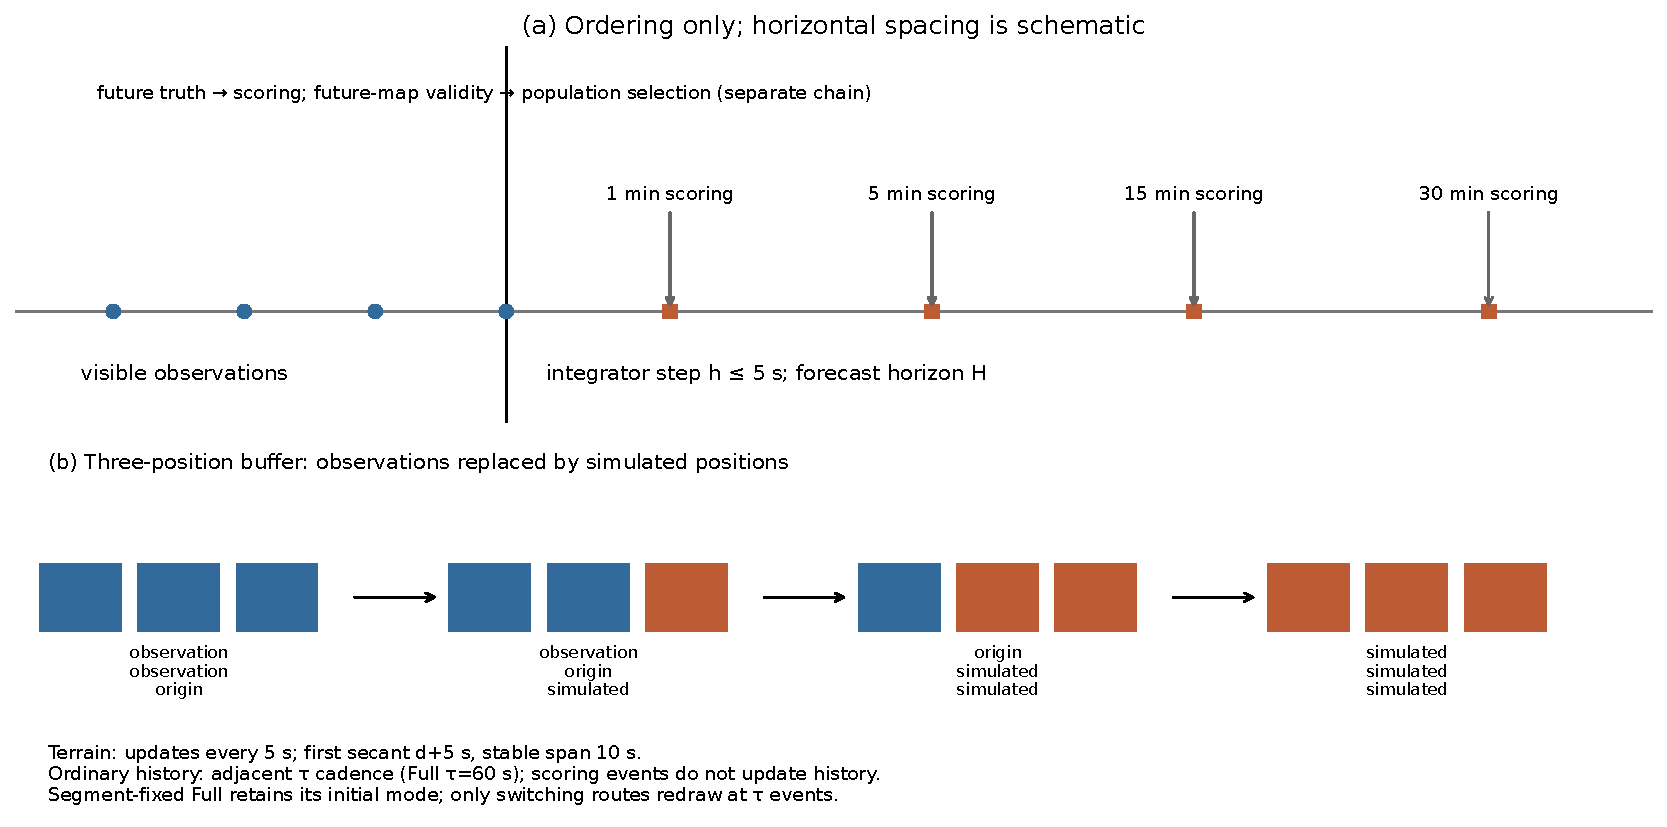
\includegraphics[width=\linewidth]{../figures/revision46-v1/revision46-history-timeline.pdf}
\caption{可见观测与模拟历史。$\tau$为观测／模型节拍，$h$为积分步长，$H$为预测时长。
地形三位置缓冲按5秒事件更新，全为模拟点后割线跨度10秒；普通Full另有$\tau=60$秒节拍。
未来观测只进入评分；评分事件本身不更新历史。图内固定英文符号与本文定义对应。}
\label{fig:history-timeline}\end{figure}

特征组为历史、保留道路子集、河流、覆盖与坡面，另含道路--覆盖、坡面--历史交互。
道路／河流方向指向最近要素点，不是道路切线或流向。
道路排除bridleway、cycleway、footway、path、pedestrian、steps、track七类，
不能解释为完整步行通行网络。坡面特征区分带符号历史、上坡与等高线方向，
方向点积不再乘坡度。几何图与十配置矩阵见\supp{fig:terrain-geometry}。

保存模型来源声明包括WorldCover 2021 v200\cite{worldcover2021}、
Overture 2026-08-19.0交通层\cite{overture202608,overtureattribution}、
HydroRIVERS v1.0\cite{hydrorivers2013,hydroriverslicense}，以及Mapzen Skadi与
Copernicus GLO-30的保留DEM产品／回退规则\cite{mapzenterrain,mapzenattribution,copernicusdem2021}。
Skadi是混合来源分发，不能认证每块瓦片均为纯NASA SRTM。
模型采样与案例显示各有来源记录；产品文档不认证逐瓦片采集年代、地图与轨迹的同期性或路线公开许可。

选中训练／验证掩码全为一，未来模拟查询却可能无效。代码对无效数值零填并附掩码，
不能据此声称已学习缺失鲁棒性。受惩罚截距与$K$个常数一掩码的最小常数子空间惩罚为
\begin{equation}\label{eq:constant-penalty}
 \min_{\sum_{j=0}^{K}a_j=c}\frac{\lambda}{2}\sum_{j=0}^{K}a_j^2
 =\frac{\lambda c^2}{2(K+1)}.
\end{equation}
base为$K=2$，all-terrain为$K=28$，分母3变29；不是全模型惩罚精确改变9.7倍。
未标准化尺度、冗余列、各配置重拟合与扩散变化进一步混杂纯信息归因。
即使预测全部成功，也只能解释配置增量，不能识别孤立地形效应。

\section{数据、目标与评价}\label{sec:data}\hypertarget{sec:protocol}{}
\subsection{事后选择的受限人群}
发布数据有12,370个窗口／1,094个记录哈希块。时间资格保留127／89，
共同特征有效保留106／73，冻结主起点选择保留46／46。
后续时长至少1,800秒的130个窗口，不等于满足全部时间规则的127个窗口。
时间合格后21窗口未通过共同地图支持；27个合格但未选块及额外窗口是选择结果，
不是预测失败。

\begin{figure}[htbp]\centering
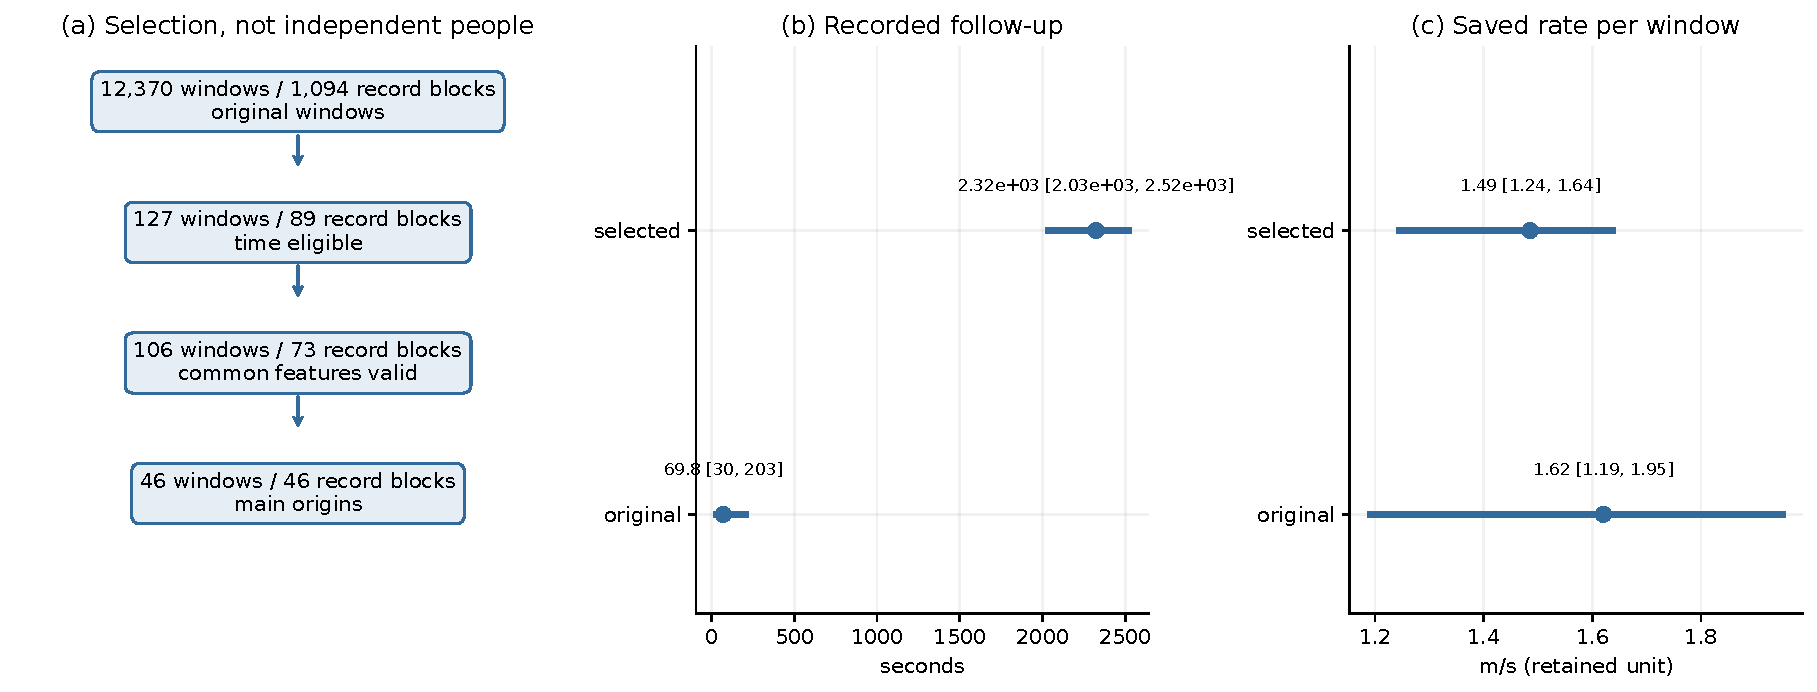
\includegraphics[width=\linewidth]{../figures/revision46-v1/revision46-population.pdf}
\caption{窗口／记录块筛选与发布前后后续时长、保存速率的中位数及四分位区间。
这是人群描述，不是预测器估计。资格检查未来真实路线地图有效性，部署时不能只凭前缀判定。}
\label{fig:population}\end{figure}

未来真位置不作为预测输入：在线查询采用模拟位置。但未来路线支持参与评估人群筛选，
这是重要事后限制。选中队列来自12国家、27来源标签，英国／比利时／卢森堡合计33/46块。
不能称全球代表性样本或部署合格队列。评估数据曾被使用，早期观察影响全部设计选择的
过程无法完整追溯，不是全新盲测留出集。

保存身份与完整序列精确检查不识别参与者、近似路线、重复访问或格式修改重复。
块重采样依赖尚未验证的独立／可交换假设。
六个known-velocity和六个point-only案例复用主记录：46独特记录块、58起点--模式案例，
不是58人或58独立块。

\subsection{保存时钟与指标定义}
预测推进到实际匹配目标，而非将观测插值到精确名义时刻。
1/5/15/30分钟目标保存经过时长范围为49--67/294--305/889--910/1785--1814秒。
R1程序重建的相对时间与预测condition tick是不同对象。
精确tick连接与datetime精度不认证物理采集时钟或UTC。
绝对偏移影响太阳／日历解释，相对尺度失真影响速率、扩散单位与真实30分钟含义。
本次不猜测时区修正。全文均指保存时钟下名义时域；$S$是日历代理，
不是经验证的日光机制。来源对账见\audit{sec:source-reconciliation-details}。

某目标时刻粒子$x_1,\ldots,x_N$与目标$y$的原有限集成评分为
\begin{equation}\label{eq:finite-es}
 \ES_N=\frac1N\sum_i\|x_i-y\|
       -\frac1{2N^2}\sum_{i,j}\|x_i-x_j\|.
\end{equation}
保留$N^2$与对角项约定，不换成$N(N-1)$。ES单位米，越低越好；加权ES为四目标等权平均。
均值位置误差$e_j=\|\bar x_j-y_j\|$，
$\mathrm{ADE}=\tfrac14\sum_{j=1}^4e_j$，$\mathrm{FDE}=e_4$。
ADE不是密集路径积分；FDE不是最佳粒子或平均粒子误差。
边际预测圆以粒子均值为圆心、粒子到均值距离的分位数为半径；
各时域分别评价覆盖和面积，不是联合路径区域。
平均面积是$\mathrm E[\pi r^2]$，不是$\pi\mathrm E[r]^2$。

终态清单为方法$28\times58\times5=8120$、地形$10\times58\times5=2900$、
同网格回放290、惯性路径58，共11,368评分槽位。
11,020登记科学预测含11,015成功和五失败；全部评分槽含11,363成功与同五失败。
槽位数不能代替数组审计范围或独立观测数。

\subsection{条件性配对推断}
先在块内平均五个固定种子，再作配对块推断；种子反映模拟变化，不是独立参与者
或训练不确定性。原同时bootstrap-$t$区间每流2,000次，族内共享块索引，
Holm零差异检验\cite{holm1979}承担另外职责。
实际界$\delta=41.100259$米来自验证惯性ES的5\%，不是已验证搜救效用界。
规划仅用三个开发块。五比较族单尾概率0.005约十个预期抽样，
四比较族约12.5个，是有限精度限制，不是同时覆盖定理\cite{davison1997}。

所有差值均为候选减具名对照，ES负差有利。跨零不是等价证据。
实际有益／有害要求原区间整体越过$-\delta$／$+\delta$且满足原统计、种子与资格门槛。
实际等价、信息不足、证据不可用、程序资格不满足是不同状态。
d2零SD别名不能独立证明功效，dt600规划功效低。
全程序与精确端点见\supp{sec:bootstrap-table-detail}。

\section{结果}\label{sec:method-results}\hypertarget{sec:method-results}{}
\subsection{先与简单外推比较：时域反转}
同主46块与原目标下，Full保存加权ES为\FullES\ 米，惯性为\InertialES\ 米。
保存差值舍入为\InertialDelta\ 米，来自未舍入值，不是相减展示均值。
1和5分钟惯性更好，15和30分钟Full更好（图\ref{fig:inertial}）。
四个离散目标不能定位精确交叉时刻。这是描述性参考比较，不是新登记优越性检验。

\begin{figure}[htbp]\centering
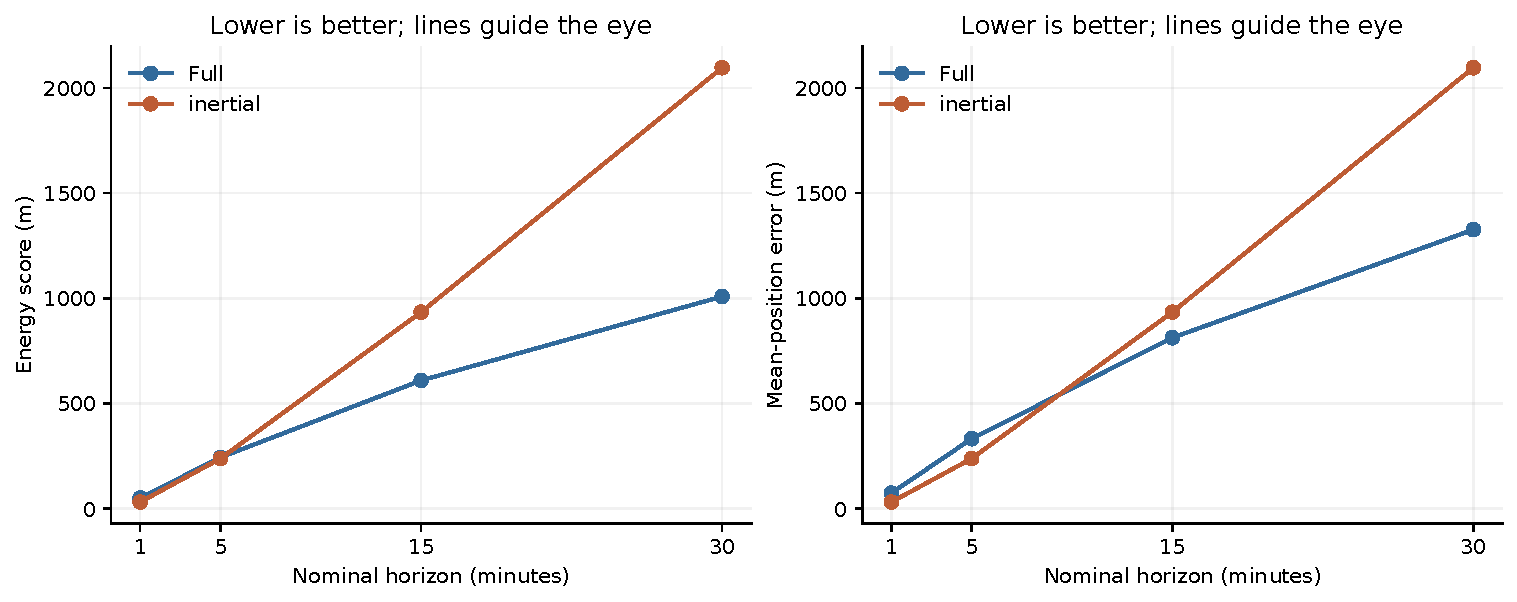
\includegraphics[width=\linewidth]{../figures/revision46-v1/revision46-inertial-horizons.pdf}
\caption{Full与确定性惯性四时域对照：左为ES，右为预测均值误差，采用原等块／等种子汇总。
连线只引导阅读，不代表连续插值或精确交叉时刻。}\label{fig:inertial}\end{figure}

\begin{table}[htbp]\centering
\caption{原目标匹配下保存预测均值误差（米）；仅四模型范围，不是ES或平均粒子误差。}
\label{tab:point-errors}
\begin{tabular}{lrrrr}\toprule
模型 & 1分钟 & 5分钟 & 15分钟 & 30分钟\\\midrule
\PointRowFull
\PointRowGMM
\PointRowdtThreeHundred
\PointRowInertial
\bottomrule\end{tabular}\end{table}
确定性参考作为点质量分布可有效比较ES，但不能检验该随机复杂结构是否必要。
任务匹配概率恒速状态空间基线是另一个未来实验，不是本稿已执行结果。

\subsection{长时域边际圆欠覆盖}
Full的四时域90\%覆盖分别为95.65\%、37.83\%、35.22\%、46.52\%。
1分钟50\%圆覆盖33.04\%，90\%圆却覆盖95.65\%；
30分钟即使95\%圆也只覆盖52.17\%。不能归结为已经证明的统一半径缩放问题。
28身份的30分钟90\%覆盖范围为21.74--79.13\%。
\begin{figure}[htbp]\centering
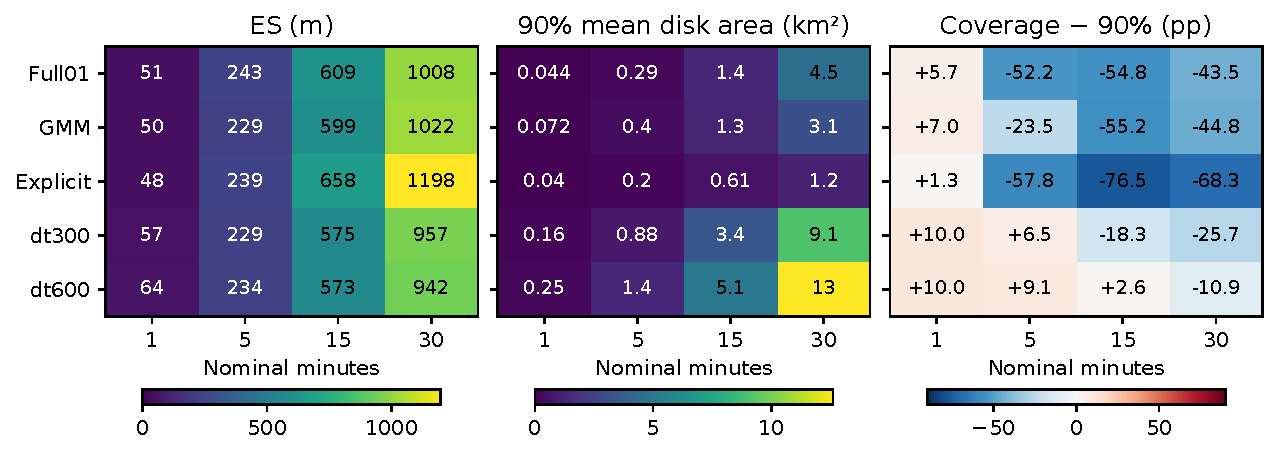
\includegraphics[width=\linewidth]{../figures/revision46-v1/revision46-selected-metric-overview.pdf}
\caption{按角色选择的概览：参考、残差混合、显式表示及长观测间隔。
行按科学角色固定，不按已见性能排名。ES与面积使用全28身份的范围；
覆盖偏差为观测减90\%的百分点，带符号数值使方向不依赖配色。}\label{fig:selected-overview}
\end{figure}
完整ES／面积／覆盖偏差概览见\supp{fig:method-overview}，发散配色以名义覆盖为中心，
不会将过覆盖视觉奖励为更好。

Full的30分钟90\%圆平均面积4.534平方千米、平均半径1183.6米，
块面积中位数4.022平方千米是另一个汇总。
300秒间隔程序平均面积9.109平方千米、覆盖64.35\%、FDE1335.73米；
600秒程序为12.609平方千米、79.13\%、1340.94米。
区域变大可覆盖更多，却未使粒子均值更准确，也未建立条件校准。
本次不根据当前评估调半径。

\subsection{组件比较与指标冲突}
21项原同时区间没有一项整体越过登记$\pm\delta$。
审计后有限算法状态为14实际等价、七证据不足；全部分辨率不变判断仍证据不足，
不意味着人类验收。pointwise相对Full01的ES增加32.95米，
GMM差为$-2.83$米且区间跨零。GMM在5和15分钟的描述性ES优势到30分钟反转。

\begin{figure}[htbp]\centering
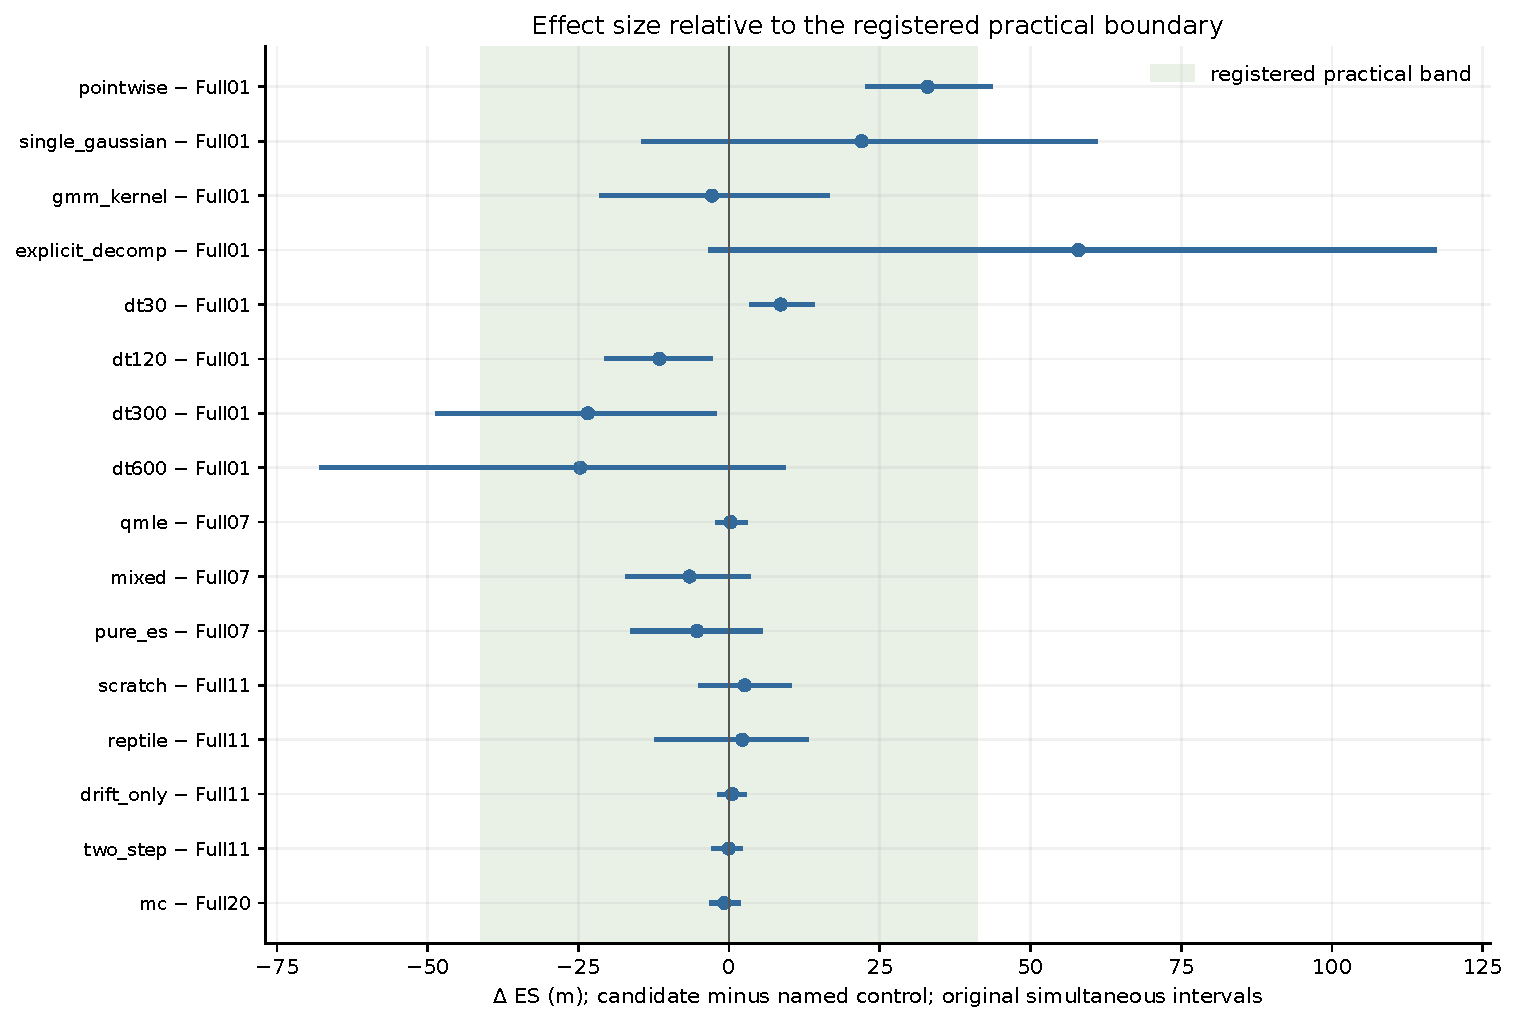
\includegraphics[width=\linewidth]{../figures/revision46-v1/revision46-practical-effects.pdf}
\caption{原配对ES效应与同时区间，保留具名候选／对照和$\pm41.10$米实际带。
微小实现一致性差值在补充材料用独立尺度显示，不删除、不解释为科学大效果。
区间位置与程序资格分别判断。}\label{fig:practical-effects}\end{figure}

ES改善可能伴随终点误差增加。补充材料按家族分面的$\Delta$ES--$\Delta$FDE四象限图
保留不同Full对照，不拼成两个独立排名。
种子／块区间图区分不确定性来源：single-Gaussian五种子差全正，块区间却为
$[-14.19,60.81]$米；GMM全负但区间$[-21.22,16.33]$米；
dt600全负但区间$[-67.65,9.08]$米。
种子方向一致不能解决人群不确定性。
完整五种子表、CRPS、终点粒子误差分位数与原120指标视图均在补充材料保留。

\subsection{地形证据与依赖失败的可用性}\label{sec:terrain-results}\hypertarget{sec:terrain-results}{}
五项保留失败有不同家族后果：F01（known-velocity dt30）使该模式观测间隔族不可用；
F02（known-velocity single Gaussian）使该模式模型结构族不可用；
F04（主all-terrain）使完整整体／LOO族不可用；
F03/F05（主LIO-river/LIO-road）使完整LIO族不可用。
整体／LOO网格1379/1380成功、一失败；LIO1148/1150成功、两失败，均无待运行缺项。
网格共享基线，不能相加为独特预测数。

原完整家族规则不允许用成功子集补因素排名。
不可用不等于无收益、零效应或等价；辅助任务完成不会消除保留失败。
五主方法家族完整，仍各有自己的资格状态。
家族／模式矩阵见\supp{fig:availability}，失败身份与日志缺口见
\audit{sec:terminal-failures}。
缺少异常栈时不能断言发散、超时、内存不足或物理断电根因。

\subsection{开发诊断与计算成本}
全地形训练拟合改善而验证拟合略差，是开发诊断，不是预测收益。
补充材料同时展示十配置MSE与原始列数／秩，区分原始缺秩与增广ridge求解成功。
拟合、正协方差或数值执行成功均不保证预测校准。

原成本实验包含15对象，各五次provider冷、一次排除预热、五次provider热，共165试验，
150次纳入延迟汇总。补充图用这些记录报告p50/p95与失败，不沿用旧单次计时推论。
provider冷不清OS缓存、不代表冷部署；五次不能认证稳定总体p95或速度--精度Pareto边界。
地图查询已经包含在rollout，不重复加总。
中断暴露记录保留并标注，不扣时、不排除、不重测。
内存采样与进程生命期峰值不能认证精确单次试验峰值。

\section{解释、局限与结论}\hypertarget{sec:discussion-score}{}
核心经验发现是时域依赖的评分、均值准确性与覆盖冲突，不能用单一赢家或一个尺度修正
概括这些预测器。校准代理与GMM标签不对应最终预测对象，观测历史与模拟历史支持不同，
未来缺图输入不同于开发输入。这些可以作为机制假说，尚不是已识别的长期欠覆盖原因。

归因另受同参数别名、未匹配模式索引、多因素程序改变及表示相关ridge惩罚限制。
细致执行记账不能修复这些设计问题；汇总复算也不能认证参与者独立、物理UTC、
无支持路线泛化或训练样本变化稳定性。
结果条件于保存拟合、选中记录、固定有限模拟与前述块重采样假设。

\subsection{真实路线案例与公开边界}\label{sec:case-horizons}\hypertarget{sec:case-horizons}{}
三个已有base/all-terrain案例与四时域路线地图仅供所有者本地审阅；
此公开稿不含地图或案例级诊断文件。原顺序、种子与预测不能证明地形效应或总体频率。
路线使用与地图图层再分发分别核实，署名或本地文件可访问不授予公开许可。
作者姓名、机构与声明仍待真实确认，不从仓库身份推断。

后续应以相同前缀与目标设计概率恒速基线、仅用开发数据选参数；
将模式匹配与参数插值分开检验；以一致分量标签校准实际多步分布；
匹配地形比较有效惩罚；核验相对／绝对时钟和独立路线／来源聚类。
这些是明确的新设计，不是本次已执行实验，也不冒充已完成的贡献前提。

RQ1支持有限实施程序比较，但登记实际界下没有已建立的实际有益／有害组件。
RQ2按完整家族规则仍不可用。
正面贡献是可复现而有边界的短长时域反转、指标取舍与严重边际欠覆盖描述，
不是已验证搜救系统、通用地形排名或新优越算法证明。
\begin{thebibliography}{99}
\bibitem{johnson2008} D. S. Johnson, J. M. London, M.-A. Lea and J. W. Durban (2008).
Continuous-time correlated random walk model for animal telemetry data.
\emph{Ecology}, 89(5), 1208--1215.
\url{https://doi.org/10.1890/07-1032.1}.
\bibitem{ghahramani2000} Z. Ghahramani and G. E. Hinton (2000).
Variational learning for switching state-space models.
\emph{Neural Computation}, 12(4), 831--864.
\url{https://doi.org/10.1162/089976600300015619}.
\bibitem{avgar2016} T. Avgar, J. R. Potts, M. A. Lewis and M. S. Boyce (2016).
Integrated step selection analysis: bridging the gap between resource selection and animal movement.
\emph{Methods in Ecology and Evolution}, 7(5), 619--630.
\url{https://doi.org/10.1111/2041-210X.12528}.
\bibitem{avgar2017correction} (2017). Corrigendum.
[Correction to Avgar et al.\ (2016)].
\emph{Methods in Ecology and Evolution}, 8(9), 1168.
\url{https://doi.org/10.1111/2041-210X.12725}.
\bibitem{gupta2018} A. Gupta, J. Johnson, L. Fei-Fei, S. Savarese and A. Alahi (2018).
Social GAN: Socially Acceptable Trajectories with Generative Adversarial Networks.
\emph{Proceedings of the IEEE Conference on Computer Vision and Pattern Recognition},
2255--2264.
\url{https://openaccess.thecvf.com/content_cvpr_2018/html/Gupta_Social_GAN_Socially_CVPR_2018_paper.html}.
\bibitem{salzmann2020} T. Salzmann, B. Ivanovic, P. Chakravarty and M. Pavone (2020).
Trajectron++: Dynamically-Feasible Trajectory Forecasting with Heterogeneous Data.
In \emph{Computer Vision -- ECCV 2020}, Lecture Notes in Computer Science,
12363, 683--700. Springer.
\url{https://doi.org/10.1007/978-3-030-58523-5_40}.
\bibitem{kidger2021} P. Kidger, J. Foster, X. Li and T. J. Lyons (2021).
Neural SDEs as Infinite-Dimensional GANs.
\emph{Proceedings of the 38th International Conference on Machine Learning},
Proceedings of Machine Learning Research, 139, 5453--5463.
\url{https://proceedings.mlr.press/v139/kidger21b.html}.
\bibitem{gao2024} T.-T. Gao, B. Barzel and G. Yan (2024).
Learning interpretable dynamics of stochastic complex systems from experimental data.
\emph{Nature Communications}, 15, 6029.
\url{https://doi.org/10.1038/s41467-024-50378-x}.
\bibitem{gneiting2007} T. Gneiting and A. E. Raftery (2007).
Strictly proper scoring rules, prediction, and estimation.
\emph{Journal of the American Statistical Association}, 102(477), 359--378.
\url{https://doi.org/10.1198/016214506000001437}.
\bibitem{gneiting2008} T. Gneiting, L. I. Stanberry, E. P. Grimit,
L. Held and N. A. Johnson (2008). Assessing probabilistic forecasts of
multivariate quantities, with an application to ensemble predictions of
surface winds. \emph{TEST}, 17, 211--235.
\url{https://doi.org/10.1007/s11749-008-0114-x}.
\bibitem{kloeden1992} P. E. Kloeden and E. Platen (1992).
\emph{Numerical Solution of Stochastic Differential Equations}. Springer.
\url{https://doi.org/10.1007/978-3-662-12616-5}.
\bibitem{nichol2018} A. Nichol, J. Achiam and J. Schulman (2018).
On First-Order Meta-Learning Algorithms. [Preprint], \emph{arXiv:1803.02999v3}.
\url{https://arxiv.org/abs/1803.02999v3}.
\bibitem{holm1979} S. Holm (1979).
A simple sequentially rejective multiple test procedure.
\emph{Scandinavian Journal of Statistics}, 6(2), 65--70.
\url{https://www.jstor.org/stable/4615733}.
\bibitem{davison1997} A. C. Davison and D. V. Hinkley (1997).
\emph{Bootstrap Methods and their Application}. Cambridge University Press.
\url{https://doi.org/10.1017/CBO9780511802843}.
\bibitem{noaa} NOAA Global Monitoring Division (n.d.).
\emph{General Solar Position Calculations}. [Online documentation]. Accessed 7 October 2026.
\url{https://gml.noaa.gov/grad/solcalc/solareqns.PDF}.
\bibitem{worldcover2021} D. Zanaga et al. (2022).
\emph{ESA WorldCover 10 m 2021 v200}. [Dataset], version v200.
\url{https://doi.org/10.5281/zenodo.7254221}.
\bibitem{overtureattribution} Overture Maps Foundation (n.d.).
\emph{Attribution and Licensing}. [Online documentation]. Accessed 6 October 2026.
\url{https://docs.overturemaps.org/attribution/}.
\bibitem{hydrorivers2013} B. Lehner and G. Grill (2013).
Global river hydrography and network routing: baseline data and new approaches
to study the world's large river systems.
\emph{Hydrological Processes}, 27(15), 2171--2186.
\url{https://doi.org/10.1002/hyp.9740}.
\bibitem{hydroriverslicense} HydroSHEDS (n.d.).
\emph{HydroRIVERS product documentation and licence}. [Online documentation], version v1.0. Accessed 6 October 2026.
\url{https://www.hydrosheds.org/products/hydrorivers}.
\bibitem{mapzenterrain} Mapzen / Tilezen (2017).
\emph{Terrain Tiles: Types of Terrain Tiles and Skadi format}.
[Dataset distribution documentation]. Document revision e3d4351; accessed 7 October 2026.
\url{https://registry.opendata.aws/terrain-tiles/}.
\url{https://github.com/tilezen/joerd/blob/e3d4351ee3e5be333e23f47cb500e9a7c310656a/docs/formats.md}.
\bibitem{mapzenattribution} Mapzen / Tilezen (2017).
\emph{Terrain Tiles: Attribution}. [Online documentation].
Document revision d8f587b; accessed 7 October 2026.
\url{https://github.com/tilezen/joerd/blob/d8f587b73d26e0a0c42cdccd9ae8c55de4197763/docs/attribution.md}.
\bibitem{copernicusdem2021} Copernicus Programme / Sinergise (2021).
\emph{Copernicus Digital Elevation Model: GLO-30 Public}.
[Dataset distribution documentation], 2021 release; accessed 7 October 2026.
\url{https://registry.opendata.aws/copernicus-dem/}.
\bibitem{overture202608} Overture Maps Foundation (2026).
\emph{2026-08-19 release notes}. [Dataset release documentation].
Data version 2026-08-19.0; accessed 7 October 2026.
\url{https://docs.overturemaps.org/blog/2026/08/19/release-notes/}.
\end{thebibliography}

\end{document}
